En este capítulo se detalla cada uno de los puntos llevados a cabo para la realización de este proyecto, empezando por definir la propuesta realizada, luego explicar el proceso ingenieril llevado a cabo y terminar desglosando el trazado de la ejecución de este proyecto.

\section{Propuesta}

El trabajo propuesto tiene como objetivo la creación de un elemento software funcional que, usando el paradigma lógico explicado en la Sección \ref{subsec:asp}, permita la generación de un escenario jugable que pueda ser ejecutado en el juego Freeciv, como se indica en la Sección \ref{subsec:freeciv}. Así mismo incluirá una interfaz gráfica interactuable que permitan al usuario marcar que zonas del terreno deben generarse y cuales no, indicando su contenido antes de lanzar el proceso de generación.

\subsection{Formato del escenario de Freeciv}

Como uno de los puntos fuerte de este trabajo tiene que ver con la generación de escenarios, este sistema tiene que tener como salida un mapa válido que sea leído correctamente por el juego Freeciv. Es por eso que explicaré en detalle el formato usado. \\

Para empezar, el formato se basa en archivo de texto plano que contiene varios campos, haciendo que sea lo más simple posible y que en la teoría se pueda modificar a mano.

\begin{lstlisting}[caption=Ejemplo de formato de mapa,label=lst:format,captionpos=b]
[scenario]
is_scenario=TRUE
name=_("My map")
description=_("This map is a example.")
players=TRUE

[savefile]
options=" +version2"
version=20
reason="Scenario"
rulesetdir="classic"
[...]

[settings]
set={"name","value","gamestart"
          "generator","SCENARIO","RANDOM"
          "mapsize","FULLSIZE","FULLSIZE"
          "maxplayers",::PLAYERS::,::PLAYERS::
          "topology","","WRAPX|ISO"
          "xsize",50,12
          "ysize",50,12
          [...]
}
set_count=9

[map]
have_huts=FALSE
t0000="h+hf  aaaa    ff"
t0001="dgg    aat    ff"
t0002="hhh           pp"
t0003="hmp        ggghh"
t0004="hmh       s dghf"
t0005=" dg      phffpm "
t0006="                "
t0007="aa     sdg    aa"
t0008="aa      h     aa"
t0009="       jff p    "
t0010="mh      s pdp pm"
t0011="gf       pdhh   "
t0012="        gpsg   p"
t0013="      h  hh     "
t0014="hff         gg s"
t0015="m+h   aaaa   m f"
startpos_count=5
startpos={"x","y","exclude","nations"
          0,2,FALSE,"Russian"
          9,11,FALSE,"Spanish"
          14,0,FALSE,""
          2,5,FALSE,""
          12,3,FALSE,""
}
b00_0000="0000000000000000"
[...]
r00_0000="0000000000000000"
[...]
\end{lstlisting}

Como se puede comprobar en el Listado \ref{lst:format}, el archivo que contiene un mapa se divide en varias secciones de datos, los cuales se marcan con un título entre corchetes. De los definidos por Freeciv, se puede destacar algunos.

\begin{itemize}
	\item \texttt{scenario}: Configura los ajustes básicos del mapa creado, como puede ser el nombre del mismo (con el campo \texttt{name}) o una breve descripción (con el campo \texttt{description}).
	\item \texttt{savefile}: Establece los valores por defecto de las opciones de juego, como puede ser la versión de Freeciv mínima (con el campo \texttt{options}), el conjunto de reglas de juego (con el campo \texttt{rulesetdir}) o las tecnologías disponibles (se establece en la lista guardada por \texttt{technology\_vector} y se indica el número de elementos en \texttt{technology\_size}).
	\item \texttt{settings}: Se puede definir una lista de valores del mapa y la topología del mismo (que se explica en detalle en la Sección \ref{subsubsec:topology}) en el campo \texttt{set}. El número de valores definidos se guarda en el campo \texttt{set\_count}.
	\item \text{map}: En esta sección se indica cada uno de los valores de terreno de la rejilla del mapa (en los campos \texttt{t00\_XXXX}), así como la lista de puntos de inicio de jugadores (definidos en la lista \texttt{startpos} e indicado el tamaño de la lista en \texttt{startpos\_count}), las capas con recursos o incluso las capas de ríos.
\end{itemize}

\subsubsection{Topología del mapa}
\label{subsubsec:topology}

El mapa es siempre una rejilla de dos dimensiones en el que cada celda es una baldosa o \textit{tile}. Esta rejilla puede estar configurada de varias maneras con la variable \texttt{topology} en la sección \texttt{settings}.

\begin{itemize}
	\item \texttt{warpx}: La topología de escenario es como un mapa terrestre, es decir el eje Este-Oeste se junta.
	\item \texttt{warpy}: La topología del escenario junta el eje Norte-Sur.
	\item \texttt{warpx warpy}: La topología del escenario es un toroide, es decir, tiene forma de donuts.
	\item \texttt{iso}: La rejilla del escenario es isométrico.
	\item \texttt{hex}: La rejilla del escenario es hexagonal.
	\item \texttt{iso hex}: La rejilla del escenario es en forma de panel de abeja.
\end{itemize}

\subsubsection{Terrenos disponibles por defecto}
\label{subsubsec:terrain}

En Freeciv, cada celda de la rejilla del mapa contiene una baldosa de terreno único, que viene definido por un identificador único, el cual puede ser uno de los siguientes:

\def\arraystretch{1.5}%  1 is the default, change whatever you need

\begin{table}[!h]
	\begin{tabular}{ p{0.7\textwidth} c c }
		\bfseries{Descripción} & \bfseries{ID} & \bfseries{Imagen} \\
		\hline
		\textit{Pradera}: Es uno de los terrenos más comunes. Las unidades se pueden mover fácilmente. & \texttt{g} & \adjustimage{height=2em,valign=t}{images/grassland.png} \\
		\textit{Llanura}: Es otro terreno muy común. Se puede usar para crear carreteras. & \texttt{p} & \adjustimage{height=2em,valign=t}{images/plains.png} \\
		\textit{Colinas}: Las unidades se mueven lentamente. Es uno de los terrenos con mayor bonus defensivo (200\%). & \texttt{h} & \adjustimage{height=2em,valign=t}{images/hills.png} \\
		\textit{Bosque}: Produce una unidad de producción (madera) con la que construir edificaciones. Tiene un bonus defensivo de 150\% & \texttt{f} & \adjustimage{height=2em,valign=t}{images/forest.png} \\
		\textit{Jungla}: Puede llegar a producir 4 unidades de producción si se encuentran con recursos de gemas o fruta. & \texttt{j} & \adjustimage{height=2em,valign=t}{images/jungle.png} \\
		\textit{Montanas}: Es el terreno con mayor bonus defensivo (300\%). Solo las unidades aéreas (aviones, cazas, etc) pueden atravesarla. & \texttt{m} & \adjustimage{height=2em,valign=t}{images/mountains.png} \\
		\textit{Desierto}: Normalmente solo se puede usar para crear carreteras, pero si hay un modificador de oasis puede generar hasta 3 unidades de producción. & \texttt{d} & \adjustimage{height=2em,valign=t}{images/desert.png} \\
		\textit{Pantano}: Se puede irrigar rápidamente. Puede producir de 5 a 9 unidades de producción si se encuentra con recursos como tundra o con especias. & \texttt{s} & \adjustimage{height=2em,valign=t}{images/swamp.png} \\
		\textit{Tundra}: Solo se pueden crear carreteras. & \texttt{t} & \adjustimage{height=2em,valign=t}{images/tundra.png} \\
		\textit{Glacier}: Ninguna de las unidades puede cruzarlo. & \texttt{a} & \adjustimage{height=2em,valign=t}{images/glacier.png} \\
		\hline
	\end{tabular}
	\caption{Tipos de terreno}\label{table:terrains1}
\end{table}

\begin{table}[!h]
	\begin{tabular}{ p{0.7\textwidth} c c }
		\bfseries{Descripción} & \bfseries{ID} & \bfseries{Imagen} \\
		\hline
		\textit{Mar}: Todas las unidades acuáticas pueden cruzarlo. Puede producir 2 unidades de producción si se encuentra con un banco de peces & & \adjustimage{height=2em,valign=t}{images/sea.png} \\
		\textit{Océano}: Solo las grandes embarcaciones y submarinos pueden pasar por encima. & \texttt{:} & \adjustimage{height=2em,valign=t}{images/ocean.png} \\
		\hline
	\end{tabular}
	\caption{Tipos de terreno}\label{table:terrains2}
\end{table}

\section{Proceso de ingeniería}

En este capítulo se explica el proceso que se ha seguido para realizar el proyecto descrito. Se empezará explicando la metodología de desarrollo escogida y a continuación se expondrá y se desgranará la gestión de este trabajo.

\subsection{Metodología de desarrollo}
\label{subsec:metodologia}

A pesar de que en un primer se ha pensado que para la planificación de este proyecto se usaría la metodología de desarrollo Scrum \cite{Schwaber:2001:ASD:559553} \cite{Schwaber:2004:APM:984028}, finalmente se ha optado por usar una amalgama entre distintas metodologías de desarrollo en espiral. Esto es debido a que Scrum tiene unas características básicas que no se han tenido en cuenta a la hora de diseñar y desarrollar el proyecto, por lo que no sería correcto decir que se ha utilizado este tipo de metodología ágil:

\begin{itemize}
	\item \textbf{Flujo de trabajo}: El trabajo se divide en varias iteraciones entre una y cuatro semanas llamadas \textit{Sprint}, en donde en cada una de ellas se obtiene un incremento funcional del producto. Al comienzo de cada iteración se realiza una reunión en donde se identifican las tareas a realizar en esa iteración, realizando una estimación de todas; durante la realización de la iteración se realiza cada día una pequeña reunión en donde se comunica el estado actual; y, al finalizar una iteración se realiza una reunión que sirve como retrospectiva y alimentación para la próxima iteración. \\
	
	A la hora de realizar este proyecto, a pesar de que se ha dividido en varias iteraciones de entre 1 semana y media, realizando una reunión al principio de estos, y en cada iteración se finaliza con un producto funcional, el resto de elementos de la metodología Scrum no se han llevado a cabo en la práctica.
	\item \textbf{Gestión de riesgos}: Uno de lo puntos de desarrollo con una metodología ágil es la de mantener una gestión de temprana de riesgos para evitar una gran desviación de la planificación. Esto se realiza mediante un panel que presenta listado ordenado de las tareas a realizar en el desarrollo total del proyecto, llamado \textit{Product backlog}. Estas tareas son las que estiman su duración y se incluyen en otro listado de tareas a realizar en cada iteración, llamado \textit{Sprint backlog}. Con esto se puede obtener una gráfica de evolución del proyecto llamado \textit{Burn down chart}, pudiendo detectar desviaciones y sobreasignaciones de forma visual debido a que también se marca el trabajo ideal de proyecto. \\
	
	Para este proyecto no se ha usado ninguno de estos elementos porque no se ha realizado un seguimiento exhaustivo del mismo a causa de la escasa experiencia de alumno a la hora de realizar una planificación y estimación del proyecto, sobre todo a la hora de seguir y diseñar un proyecto con una metodología de desarrollo ágil.
\end{itemize}

Debido a todos estos factores expuestos, se podría indicar que la metodología usada finalmente está más cerca de una basada en modelos de prototipos en donde se tiene en cuenta que cada prototipo resultante de una iteración es un modelo funcional del mismo, y en donde es revisado en la reunión de la siguiente iteración sin estar presente el cliente final, si no que solo con el director del proyecto. También en esta reunión se definen las tareas a realizar para el desarrollo del proyecto de cara a la nueva iteración. \\

\subsection{Gestión del proyecto}
\label{subsec:gestion}

A continuación se describirá la planificación llevada a cabo para cumplir con el tiempo estimado de realización del proyecto, así como el coste y los recursos necesarios para la construcción del mismo.

\subsubsection{Planificación}

Volviendo a lo comentado en la Sección \ref{subsec:metodologia}, con respecto la planificación del desarrollo del trabajo en cuestión, se ha dividido en varias iteraciones que han ido incrementando las funcionalidades del producto final. Estas iteraciones vienen expresados de una forma gráfica en la Figura \ref{fig:gantt} y explicados en detalle en la Tabla \ref{table:iteraciones}.

\begin{figure}[!h]
	\centering
	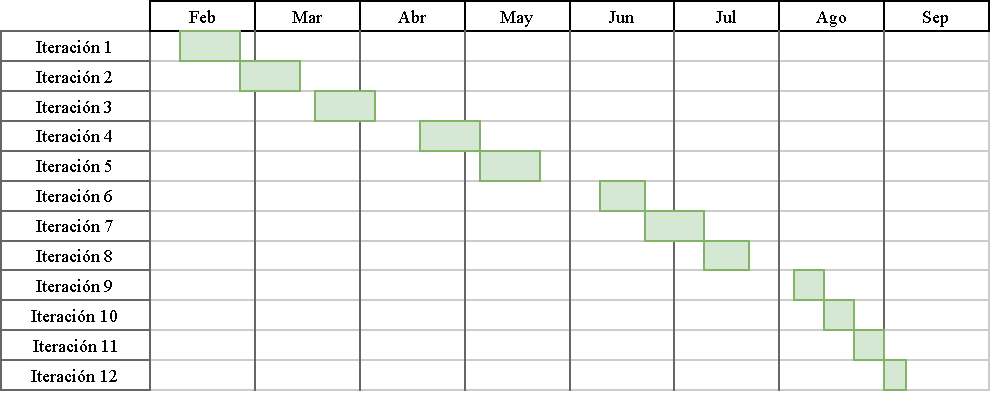
\includegraphics[width=\textwidth]{images/gantt.pdf}
	\caption{Diagrama de Gantt con las iteraciones del proyecto}
	\label{fig:gantt}
\end{figure}

Cabe destacar que el proyecto en cuestión ha tenido dos aproximaciones diferentes. La primera aproximación tiene que ver con las iteraciones 1-3, en donde el sistema generaba todos los tipos de terrenos del mapa. El problema de esta aproximación es que ocasionaba que la generación de mapa tardase mucho más de lo que alguien puede considerar razonable. Esto es debido a la naturaleza de ASP, que tal como se describe en la Sección \ref{subsec:asp}, provoca que el conjunto de reglas a tener en cuenta sea exponencial, dando como resultado una explosión combinatoria de hechos y que la herramienta no sea usable. \\

\def\arraystretch{1}%  1 is the default, change whatever you need

\begin{table}
	\centering
	\begin{tabular}{ c c }
		\bfseries{Iteración} & \bfseries{Tiempo (h)} \\
		\hline
		1 & 30 \\
		2 & 30 \\
		3 & 30 \\
		4 & 20 \\
		5 & 20 \\
		6 & 32 \\
		7 & 32 \\
		8 & 32 \\
		9 & 32 \\
		10 & 32 \\
		11 & 32 \\
		12 & 40 \\
		\hline
		\bfseries{Total} & 362 \\
		\hline
	\end{tabular}
	\caption{Desglose de las iteraciones}\label{table:iteraciones}
\end{table}

Como segunda aproximación, la cual comprende el resto de iteraciones, se ha decidido dividir el programa en distintos módulos independientes que se encargan de generar distintas partes del mapa. Esto hace que el tiempo sea mucho más razonable y sea más manejable. Aún así, el hecho de cambiar de aproximación, como puede entenderse, hizo que se tuviera que cambiar la parte declarativa de la herramienta.

\subsubsection{Coste y recursos}

Para calcular el coste de los recursos humanos que ha supuesto este proyecto, además de las 362 horas totales del proyecto, también se han llevado a cabo reuniones de una hora a la hora de iniciar cada iteración, así como una al inicial el proyecto y otra al terminar el mismo, dando un total de 14 horas a mayores al proyecto. Teniendo esto en cuenta y siguiendo la Guía Salarial del Sector TI en Galicia \cite{guiasalarial}, se ha estimado los costes que se pueden ven en la Tabla \ref{table:costehumano}.

\begin{table}[!h]
	\centering
	\begin{tabular}{ c c c c }
		\bfseries{Recurso} & \bfseries{Tiempo (h)} & \bfseries{Coste (\euro/h)} & \bfseries{Total} \\
		\hline
		Doctor Investigador & 14 & 24,00 & 336,00 \\
		Analista Programador & 376 & 9,00 & 3384,00 \\
		\hline
		\bfseries{Total} & 376 & & 3720,00 \\
		\hline
	\end{tabular}
	\caption{Coste de los recursos humanos del proyecto}\label{table:costehumano}
\end{table}

\begin{table}[!h]
	\centering
	\begin{tabularx}{\textwidth}{ X X X X X }
		\bfseries{Recurso} & \bfseries{Vida (mes)} & \bfseries{Uso (mes)} & \bfseries{Coste (\euro)} & \bfseries{Total (\euro)} \\
		\hline
		Portátil & 48 & 7 & 800,00 & 116,67 \\
		Freeciv & $\infty$ & 7 & - & 0 \\
		Clingo & $\infty$ & 7 & - & 0 \\
		LÖVE & $\infty$ & 7 & - & 0 \\
		HUMP & $\infty$ & 7 & - & 0 \\
		SUIT & $\infty$ & 7 & - & 0 \\
		json.lua & $\infty$ & 7 & - & 0 \\
		busted & $\infty$ & 7 & - & 0 \\
		luaproc & $\infty$ & 7 & - & 0 \\
		LDoc & $\infty$ & 7 & - & 0 \\
		Github & $\infty$ & 7 & - & 0 \\
		Travis-CI & $\infty$ & 7 & - & 0 \\
		Coveralls & $\infty$ & 7 & - & 0 \\
		LaTeX & $\infty$ & 7 & - & 0 \\
		\hline
		\bfseries{Total} & & & & 116,67 \\
		\hline
	\end{tabularx}
	\caption{Coste de los recursos humanos del proyecto}\label{table:costematerial}
\end{table}

Por otro lado, en la \ref{table:costematerial} se recoge la lista de recursos materiales y lógicos necesarios para el desarrollo de este proyecto. Para el caso de los recursos \textit{hardware} se ha tenido en cuenta el tiempo de uso para este proyecto con respecto a su vida útil, mientras para los recursos \textit{software}, se ha preferido por usar herramientas y bibliotecas de uso libre y gratuitas, de ahí que el coste no esté contado para el resultado final. \\

Con todo esto se puede concluir que el coste total del proyecto asciende hasta \EUR{3836,67} en total.

\section{Análisis del software}

Una vez definido el sistema y planificada su construcción, se ha realizado un análisis en donde se identifican los requisitos que debe cumplir el software una vez terminado el proyecto.

\subsection{Requisitos funcionales}
\label{subsec:funcrequirements}

Los requisitos funcionales son aquellas condiciones indispensables que estipulan las funcionalidades que debe proporcional el sistema. Para este proyecto se ha recogido los diferentes requisitos:

\begin{itemize}
	\item Generación de un mapa que sea legible por el videojuego Freeciv.
	\item Permitir añadir restricciones sobre ciertas zonas del mapa.
	\item Poder guardar y recuperar el mapa en un formato sencillo.
\end{itemize}

\subsection{Requisitos no funcionales}

Los requisitos no funcionales, por su contra, son aquellas condiciones indispensables que debe cumplir el sistema a la hora de diseñar e implementar. Para este proyecto se han tenido en cuenta estos requisitos:

\begin{itemize}
	\item Eficiencia y eficacia: El generador debe responder en el menor tiempo posible arrojando una respuesta óptima.
	\item Escalabilidad: El generador debe trabajar con mapas de diferentes tamaños, por lo que el sistema debe poder soportar cualquier tamaño de entrada.
	\item Usabilidad: La interfaz gráfica debe ser lo más sencilla posible, evitando que el usuario tenga que realizar tareas tediosas a la hora de construir mapas.
\end{itemize}

\section{Diseño del sistema}

Una vez definidos los requisitos se ha procedido a realizar el diseño software del sistema en cuestión, empezando a concretar la arquitectura propuesta y luego desarrollando los casos de uso y diagramas de clases.

\subsection{Arquitectura software}
\label{subsec:arquitectura}

Debido a que el sistema cuenta con una interfaz gráfica y un módulo que se encargará de generar el mapa, el sistema estará dividido en dos partes concretas tal y como se puede ver en la Figura \ref{fig:arquitectura}:

\begin{itemize}
	\item Una parte que será la aplicación gráfica, que actuará en todo momento como \textit{Front-end} de cara al usuario. Esta parte sigue la estructura Modelo-Vista-Controlador (MVC), en donde el controlador se encargará de hacer de puente entre la interfaz gráfica, que es lo que manipulará el usuario, y los datos guardados en memoria. Así mismo proporcionará las funcionalidades básicas del sistema como guardar o cargar el mapa y crear un mapa en blanco.
	\item La segunda parte actuará como \textit{Back-end}, que se encargará de generar el mapa mediante un programa lógico escrito en ASP que se ejecutará Clingo. Contiene un controlador que se encargará de hacer la llamada a Clingo y de obtener su resultado, y luego otro controlador que se encargará de llamar primeramente al programa lógico que genere las regiones y luego, dada una región, rellene las casillas de la región. Para ello primeramente define que zonas son tierra y que zonas son agua, y con las zonas con tierra se rellenan con cordilleras y con áreas bióticas (las cuales son zonas grandes que contienen un solo tipo de terreno). Una vez realizado terminará generando los mares y los puntos de inicio para los jugadores.
\end{itemize}

\begin{figure}[!h]
	\centering
	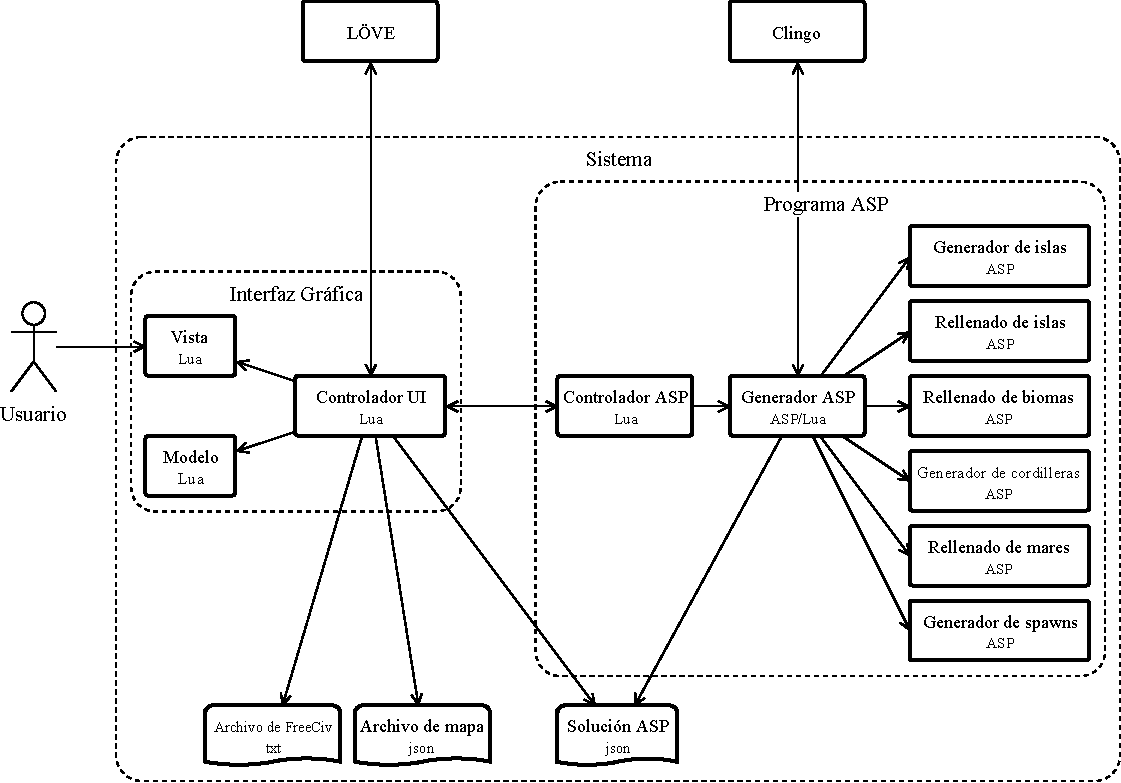
\includegraphics[width=\textwidth]{images/arquitectura.pdf}
	\caption{Arquitectura del sistema}
	\label{fig:arquitectura}
\end{figure}

Tanto el controlador de la interfaz de usuario como el controlador del programa ASP se ejecutarán en paralelo, pudiendo enviarse información de un controlador a otro para saber cuando hay que empezar una generación o si esta terminó. A pesar de esto, los resultados de la generación de ASP se guadarán en un archivo intermedio para evitar enviar gran cantidad de datos entre los elementos.

\subsection{Casos de uso}
\label{subsec:cases}

El sistema tiene en cuenta que se usará en todo momento por un único usuario, el cual llevará a cabo todas las funcionalidades propuestas en la Sección \ref{subsec:funcrequirements} a través de una interfaz gráfica que se explica en la Sección \ref{subsec:mockups}. Estos requisitos funcionales se transforman, por tanto, en los casos de uso del sistema que se proponen el la Figura \ref{fig:cases}.

\begin{figure}[!h]
	\centering
	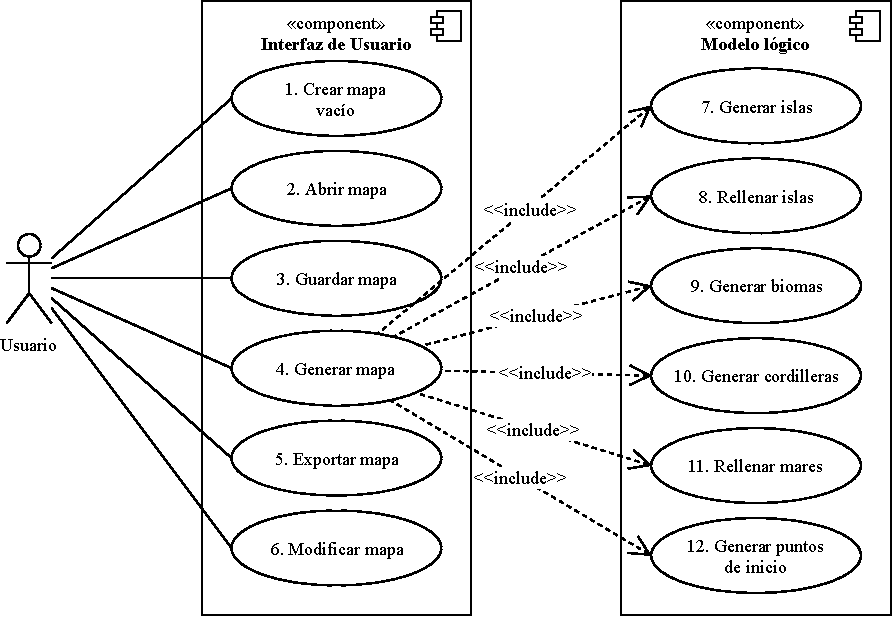
\includegraphics[width=\textwidth]{images/casos-de-uso.pdf}
	\caption{Casos de uso del sistema propuesto}
	\label{fig:cases}
\end{figure}

\subsection{Pantallas del sistema}
\label{subsec:mockups}

El proyecto propuesto está pensado para ser usado a través de una interfaz gráfica de usuario, la cual es modelada mediante un patrón MVC como se indica en la Sección \ref{subsec:arquitectura}. Esta interfaz está dividida en varias vistas, las cuales corresponden con los casos de uso propuestos contra los que el usuario interacciona directamente en la Sección \ref{subsec:cases}.

\begin{itemize}	
	\begin{figure}[!h]
		\centering
		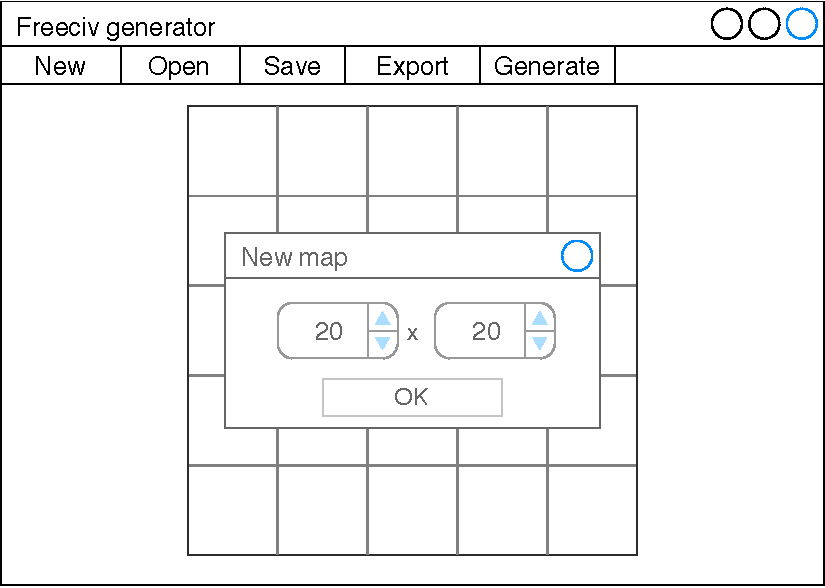
\includegraphics[width=0.5\textwidth]{images/new-map.pdf}
		\caption{Pantalla de nuevo mapa}
		\label{fig:newmock}
	\end{figure}
	
	\item 1. Crear mapa vacío: Se acciona cuando el usuario presiona en el botón de ``Crear mapa'' en la barra de herramientas, lo que despliega una ventana emergente parecida a la Figura \ref{fig:newmock}. Aquí el usuario puede indicar el tamaño del mapa a crear y pulsar el botón de ``Aceptar''. Con esto el sistema muestra una rejilla vacía.

	\begin{figure}[!h]
		\centering
		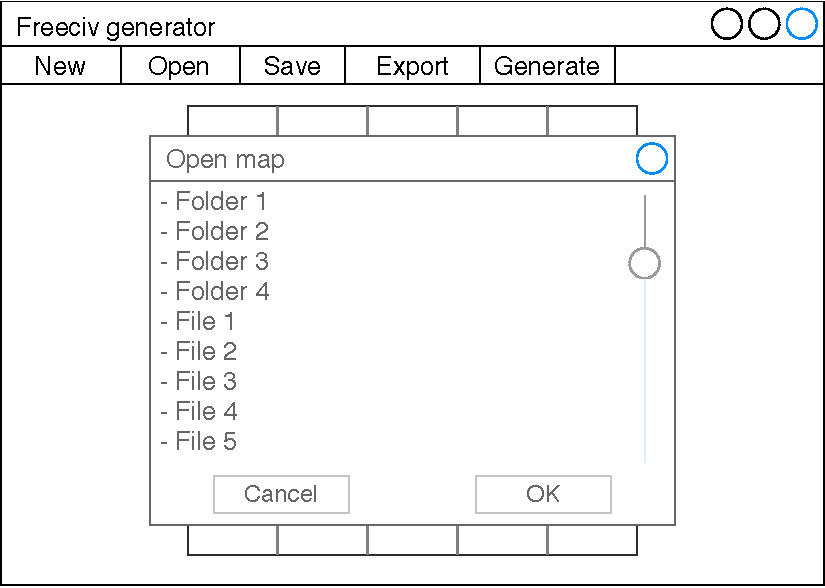
\includegraphics[width=0.5\textwidth]{images/open-map.pdf}
		\caption{Pantalla de abrir archivo de mapa}
		\label{fig:openmock}
	\end{figure}

	\item 2. Abrir mapa guardado en disco: Se inicia cuando el usuario presiona en el botón de ``Abrir mapa'' en la barra de herramientas, lo que despliega una ventana emergente parecida a la Figura \ref{fig:openmock}. Aquí el usuario navega a través de una lista que representa los archivos guardados en disco y selecciona un archivo anteriormente guardado por la aplicación que representa un mapa. El sistema procede a cargarlo y mostrar los datos del mapa en la rejilla principal.
	
	\begin{figure}[!h]
		\centering
		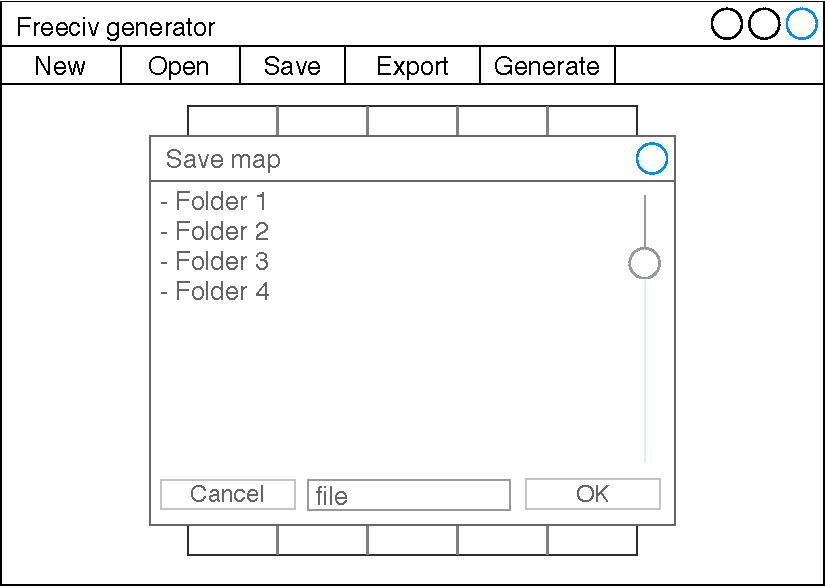
\includegraphics[width=0.5\textwidth]{images/save-map.pdf}
		\caption{Pantalla de guardar mapa}
		\label{fig:savemock}
	\end{figure}
	
	\item 3. Guardar mapa en disco: Se inicia cuando el usuario presiona en el botón de ``Guardar mapa'' en la barra de herramientas, mostrando una ventana emergente como la de la Figura \ref{fig:savemock}. Aquí el usuario navega por las carpetas guardadas en disco a través de una lista y selecciona una donde se guardará. Además, escribe el nombre del nuevo archivo en un campo de texto debajo de esta lista y acepta. El sistema procede a transformar los datos del mapa en un fichero que se guarda en disco donde el usuario indicó.
	
	\begin{figure}[!h]
		\centering
		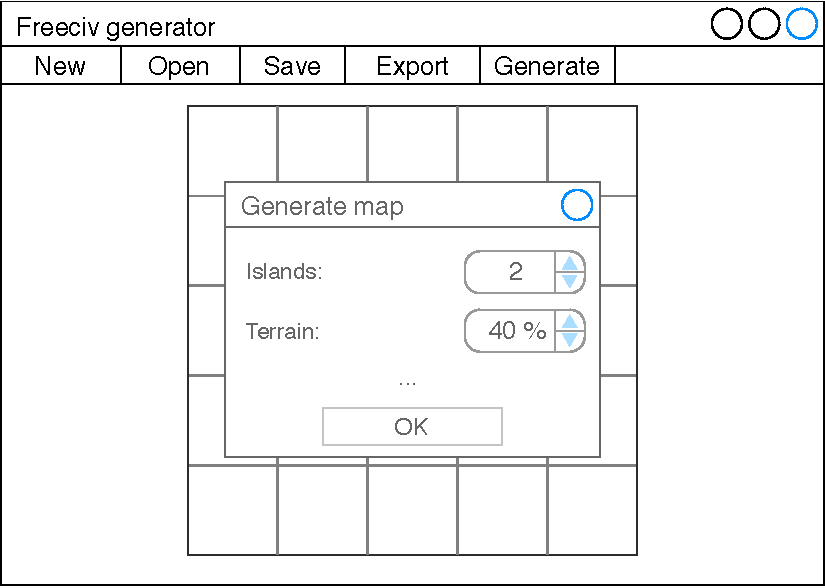
\includegraphics[width=0.5\textwidth]{images/generate-map.pdf}
		\caption{Pantalla de generar mapa}
		\label{fig:generatemock}
	\end{figure}
	
	\item 4. Generar mapa: Se inicia cuando el usuario acciona el botón de ``Generar mapa'' en la barra de herramientas, haciendo que el sistema muestre una ventana emergente parecida a la Figura \ref{fig:generatemock}. Aquí el usuario indica los parámetros que prefiera en la generación y acepta. En sistema procede a llamar a la parte del programa lógico creado en ASP, la cual va ejecutando cada uno de los casos de uso. Entre medias, el sistema lanza una vista como la de la Figura \ref{fig:waitingmock} para proporcionar retro-alimentación al usuario. Una vez acabada la generación, el sistema muestra en la rejilla principal con el mapa que se ha generado finalmente.

	\begin{figure}[!h]
		\centering
		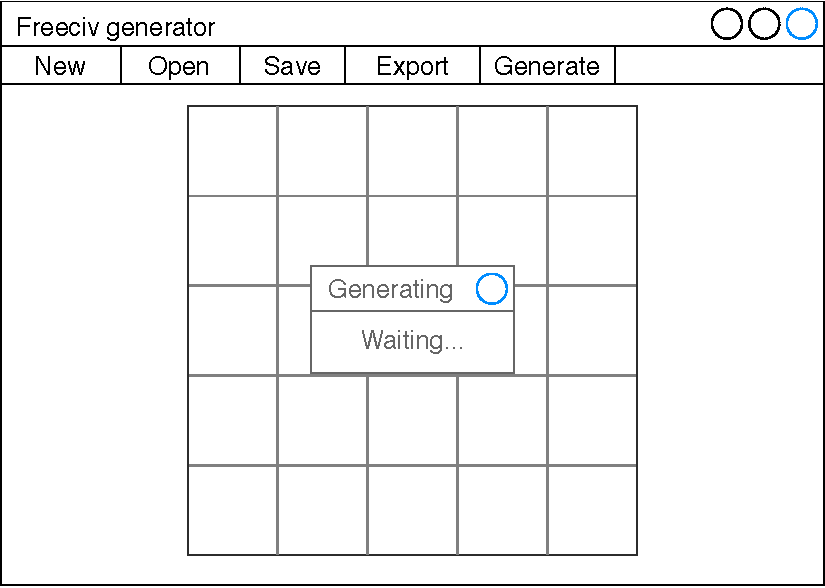
\includegraphics[width=0.5\textwidth]{images/waiting-mock.pdf}
		\caption{Pantalla con el mensaje de espera}
		\label{fig:waitingmock}
	\end{figure}
	
	\item 5. Exportar mapa al formato de Freeciv: Se inicia cuando el usuario presiona en el botón de ``Exportar mapa'' en la barra de herramientas, mostrando una ventana emergente como la de la Figura \ref{fig:exportmock}. Aquí el usuario navega por las carpetas guardadas en disco a través de una lista y selecciona una donde se guardará. Además, escribe el nombre del nuevo archivo en un campo de texto debajo de esta lista y acepta. El sistema procede a transformar los datos del mapa en un fichero reconocible por Freeciv y se guarda en disco donde el usuario indicó.
	
	\begin{figure}[!h]
		\centering
		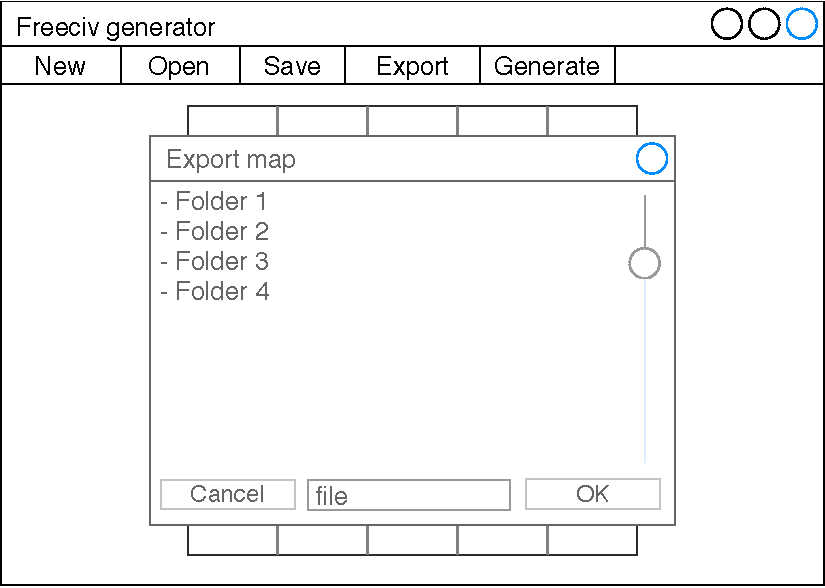
\includegraphics[width=0.5\textwidth]{images/export-map.pdf}
		\caption{Pantalla de exportar mapa}
		\label{fig:exportmock}
	\end{figure}
	
	\item 6. Modificar mapa: Se inicia cuando el usuario presiona sobre una de las celdas de la rejilla expuesta en la Figura \ref{fig:mainmock}. El sistema pasará a cambiar el terreno de la celda por otro, realizando un ciclo en el momento en el que no quede ninguna opción nueva.
	
	\begin{figure}[!h]
		\centering
		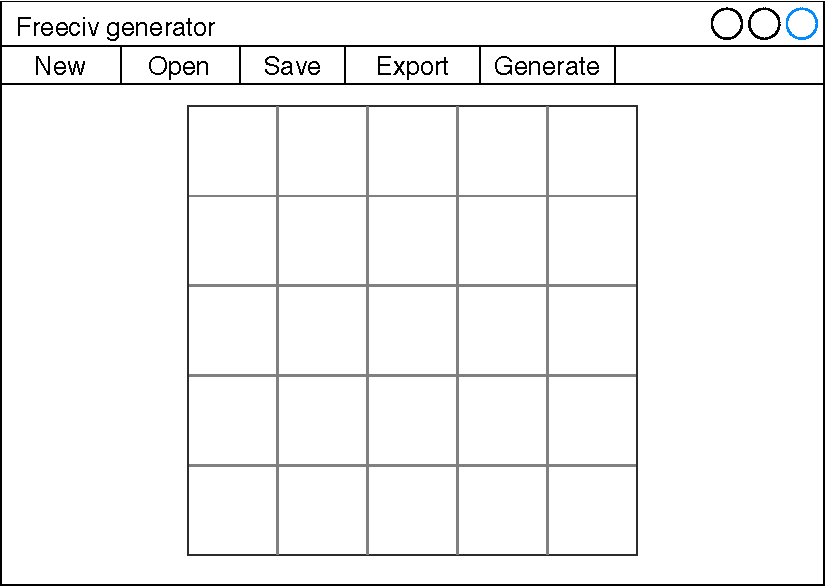
\includegraphics[width=0.5\textwidth]{images/aplicacion.pdf}
		\caption{Pantalla principal de la aplicación}
		\label{fig:mainmock}
	\end{figure}

\end{itemize}

\subsection{Diseño del programa lógico}
\label{subsubsec:generator}

Retornando a lo comentado en la Sección \ref{subsec:arquitectura}, una de las piezas fundamentales de este proyecto es la definición de un generador de mapas en formato declarativo. Este módulo está pensado mediante el paradigma de programación lógica que usa la tecnología ASP, tal y como se expone en la Sección \ref{subsec:asp}. \\

El objetivo de este generador es intentar dar un modelo declarativo basado en reglas que corresponda en mayor o menor medida con la definición de un mapa de Freeciv. Es por esto que, como se ha contado en la Sección \ref{subsec:gestion}, para evitar los problemas que puede suponer este proyecto en cuanto a evitar tener una explosión combinatoria de soluciones válidas, se ha decidido finalmente realizar una aproximación dividiendo este módulo en varios programas independientes que generan partes concretas del escenario. \\

\subsubsection{Generación de regiones}
\label{subsubsec:regiones}

Como primer paso para la generación del mapa, se ha pensado en usar un programa lógico que, dada una división grande del mapa (la cual llamaremos cuadrante), identifica para cada una de ellas a que región o isla pertenece, tal y como se puede ver en la Figura \ref{fig:regiones}.

\begin{figure}[!h]
	\centering
	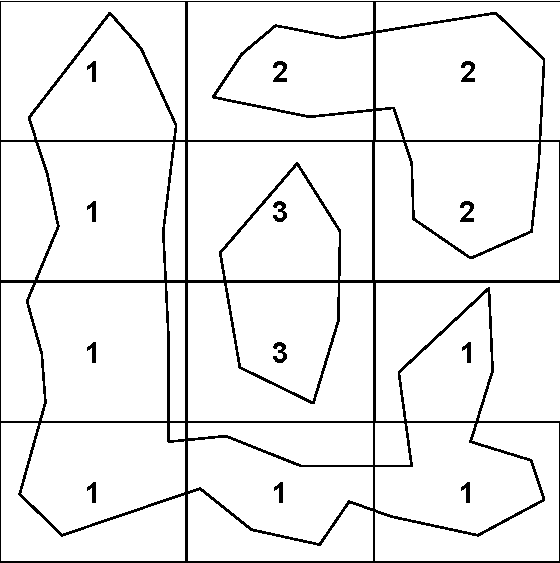
\includegraphics[width=0.4\textwidth]{images/regiones.pdf}
	\caption{Ejemplo de mapa dividido en cuadrantes}
	\label{fig:regiones}
\end{figure}

Para ello elige un cuadrante único para isla, el cual va a ser la raíz desde donde se vaya expandiendo toda la región. Esto se ha implementado mediante siguientes reglas, en donde primeramente se selecciona una raíz dado un cuadrante y se prohíbe que dos raíces de distintos cuadrantes tengan la misma posición: \\

\begin{lstlisting}[label=lst:qroot]
1 { q_root(C, I): q_pos(C) } 1 :- region(I).
:- q_root(C, I), q_root(C, J), I!=J.
\end{lstlisting}

\hspace{1em}

Para que cada raíz se expanda por el mapa, se ha planteado que las celdas contiguas sean alcanzables, es decir, que si está adyacente (se tiene en cuenta 4-adyacente) a la raíz o a otra celda conectada a la raíz, esta pueda o no ser alcanzada siempre que no se haya escogido para otra región. Esto en ASP se traduce en estas reglas: \\

\begin{lstlisting}[label=lst:qreached]
q_reached(C, I) :- q_root(C, I).
{q_reached(C, I)} :- q_reached(D, I), region(I), 
   not existsanother(I, C), q_adj(D, C).
existsanother(I, C) :- q_reached(C, J), region(J), region(I),
   J!=I.
\end{lstlisting}

\hspace{1em}

Finalmente, para que todo el mapa esté completo y no haya cuadrantes sin definir a una región, se ha añadido una restricción que evita las soluciones en donde el número de elementos \texttt{q\_reached} no es igual al máximo número de cuadrantes: \\

\begin{lstlisting}[label=lst:qmax]
n_quadrants(Z) :- #count{C, I: q_reached(C,I)} = Z.
:- n_quadrants(Z), max_quadrants(MAX), Z!=MAX.
\end{lstlisting}

\subsubsection{Definición de regiones}
\label{subsubsec:cuadrantes}

Como segundo paso que se realiza, se procede a detallar cada una de las regiones por separado, indicando qué celdas del mapa que corresponde a esa región son de agua y cuales son de tierra. Para ello se realiza una aproximación parecida explicada en la generación de regiones, en donde se toma una celda que cae dentro de la región como celda raíz que contendrá tierra: \\

\begin{lstlisting}[label=lst:croot]
1 {rootcell(P) : c_pos(P)} 1.
\end{lstlisting}

\hspace{1em}

Con esto la celda raíz de la isla intenta alcanzar al resto de celdas adyacentes usando una definición similar a la explicada en el apartado anterior: \\

\begin{lstlisting}[label=lst:croot]
reached(P) :- rootcell(P).
{reached(P)} :- reached(Q), adj(Q, P).
\end{lstlisting}

\hspace{1em}

Aún así, en este caso no queremos que la tierra rellene completamente la isla, el tamaño de la selección de celdas viene condicionado por una constante que indica la cantidad de tierra que se tiene que alcanzar. Por defecto está establecida para un 20\% del número de celdas totales de la región: \\

\begin{lstlisting}[label=lst:cmax]
cells_reached(Z) :- #count{P: reached(P)}=Z.
:- cells_reached(Z), n_cells(MAX), dims(ROWS, COLS, LAND),
   Z!=MAX*LAND/100.
\end{lstlisting}

\hspace{1em}

Cabe destacar que en este apartado también se han añadido restricciones evitar la generación de formas o zonas que no sean del todo creíbles. Estas restricciones son las siguientes y pueden comentarse en cualquier momento sin peligrar el resto del programa: \\

\begin{lstlisting}[label=lst:crestriccions]
% Forbidden create lakes with 1 cell
:- c_pos(P), not reached(P), top(P, T), T!=w, left(P,L), L!=w,
   bottom(P,B), B!=w, right(P,R), R!=w.

% Forbidden create bridges
:- reached(P), top(P, w), left(P, L), L!=w, bottom(P, w),
   right(P, R), R!=w.
:- reached(P), top(P, T), T!=w, left(P, w), bottom(P, B), B!=w,
   right(P,w).
\end{lstlisting}

\hspace{1em}

Finalmente hay que destacar que, como la generación de regiones es independiente, para evitar que las islas de tierra se solapen, el programa principal genera unas restricciones que corresponden con las celdas adyacentes a las que están en borde de una región y han sido seleccionadas como tierra. Estas restricciones se tienen en cuenta en la siguiente generación, evitando que esto suceda.

\subsubsection{Rellenado del terreno}

Una vez se ha terminado la ejecución del apartado anterior, se procede a la selección de los biomas, es decir, las zonas de tierra con un tipo de terreno en concreto, que contendrá esa región. Para ello, de un modo similar al que se viene explicando, se elige una celda que será la raíz del bioma y se extiende mediante las celdas adyacentes. Aún así hay que destacar que, por defecto, el bioma de una celda de tierra es de hierba, por lo tanto aquí caben dos afirmaciones que se han supuesto en esta generación:

\begin{itemize}
	\item La hierba es el único bioma que no se genera, si no que todas las celdas contienen hierba a siempre y cuando no se exprese lo contrario.
	\item Puede existir islas que no tengan todos los tipos de biomas, por lo que puede o no generarse un tipo concreto de bioma.
\end{itemize}

Con esta información se han llevado a cabo las siguiente reglas: \\

\begin{lstlisting}[label=lst:biomas]
% The root of a bioma
{root(P, T) : cell(P, l)} :- biomas(T).
:- root(P, T), root(P, U), T!=U.

% Defines which cells could be reached
reached(P, T) :- root(P, T).
{reached(P, T)} :- biomas(T), cell(P, l), adj(P, Q),
   reached(Q, T).
:- reached(P, T), reached(P, U), T!=U.
\end{lstlisting}

\hspace{1em}

Por otra parte, pueden existir ciertos biomas que solo se generen en una latitudes concretas, como los casquetes polares. Para ello se pueden crear ciertas reglas especiales que generen estos terrenos en función de la fila del mapa en la que se encuentra. En el siguiente ejemplo se ha recogido las reglas que generarían los casquetes en la zona norte y en la zona sur del mapa, siendo de ancho un 10\% del alto del mapa: \\

\begin{lstlisting}[label=lst:glaciers]
ice(ROWS*10/100) :- dims(ROWS, COLS, TERRAIN).

land(p(X, Y), glacier) :- cell(p(X, Y), l), ice(N), X < N-1.
land(p(X, Y), glacier) :- cell(p(X, Y), l), ice(N),
   dims(ROWS, COLS, TERRAIN), X > ROWS-N-1.
\end{lstlisting}

\hspace{1em}

Para terminar con este apartado, se ha añadido varias restricciones de tamaño. Las primeras reglas tienen que ver con la cantidad de tipos de terrenos generados, la cual sigue con el esquema propuesto en el apartado anterior (por defecto está establecida para un 20\% del número de celdas totales de la región): \\

\begin{lstlisting}[label=lst:tmax]
n_cells(Z) :- #count{C, I : reached(C, I)} = Z.
:- n_cells(Z), max_cells(MAX), dims(ROWS, COLS, TERRAIN),
   Z!=MAX*TERRAIN/100.
\end{lstlisting}

\hspace{1em}

Finalmente se ha decidido que un bioma tiene que ocupar al menos dos casillas. Debido a eso, para los biomas generados se cuenta el número de celdas alcanzadas y se añade una restricción que evita que esta cuenta sea menor a dos celdas: \\

\begin{lstlisting}[label=lst:tmax]
size_bioma(T, N) :- root(Q, T), cell(Q, l), 
   #count{P: reached(P, T)} = N.
:- size_bioma(T, N), N < 2.
\end{lstlisting}

\subsubsection{Definición de cordilleras}

Para la definición de cordilleras (el tipo de terreno montaña), esta se realiza una vez se ha completado la definición de los biomas de una isla, evitando así que el módulo anterior tenga una explosión combinatoria fuerte de resultados. Así mismo, esto nos permite tener en cuenta que, para dar un mayor realismo a la generación, en la vida real puede existir un sistema montañoso que divida ecosistemas con el mismo tipo de bioma debido al acercamiento de dos placas tectónicas. \\

Después de esta breve explicación, para la definición de las reglas de generación de cordilleras se ha propuesto que esta generación tenga dos puntos, un punto inicial y un punto final que comprenda el inicio y el final de la coordillera: \\

\begin{lstlisting}[label=lst:pointsystem]
% Generate the start and the end position
1 {start(P) : cell(P, l)} 1.
1 {end(P) : cell(P, l)} 1 :- start(Q).
% Forbidden that start and end points are the same.
:- start(P), end(Q), P==Q.
\end{lstlisting}

\hspace{1em}

Con esto lo que se pretende es hacer un camino que vaya de un punto a otro, para ello, de la misma forma que se ha generado las islas, se parte del punto inicial y se van alcanzando las celdas de tierra adyacentes: \\

\begin{lstlisting}[label=lst:mreached]
% The start cell is reached always.
reached(P) :- start(P).
% A cell next to a reached cell could be reached
{reached(P)} :- cell(P, l), reached(Q), adj(P, Q).
\end{lstlisting}

\hspace{1em}

Lo siguiente es evitar todas las soluciones en donde no se haya alcanzado el punto final, para ello se define el átomo \texttt{complete} en función de esto y se prohibe las soluciones que no tienen este átomo: \\

\begin{lstlisting}[label=lst:mend]
% The path is complete if the end is reached.
complete :- end(P), reached(P).
% Forbidden the paths that don't reach the end point.
:- not complete.
\end{lstlisting}

\hspace{1em}

Con esto generará un camino de coordilleras con cualquier ancho. Aún así se ha preferido acotar este camino a un ancho máximo. Para ello se han añadido unas reglas para obtener el número de vecinos adyacentes, en donde se parte de un borde del camino que tiene valor 0 y se avanza en un sentido, por ejemplo, partiendo de un borde, sus vecinos adyacentes hacia arriba serían: \\

\begin{lstlisting}[label=lst:msizedef]
size(p(X, Y), up, 0) :- reached(p(X, Y)), not reached(p(X-1, Y)).
size(p(X, Y), up, N+1) :- reached(p(X, Y)), size(p(X-1, Y), up, N).
\end{lstlisting}

\hspace{1em}

Esto se realiza para todos los sentidos correspondientes a la definición de adyacencia (arriba, abajo, izquierda y derecha). Con esto se puede obtener el ancho del camino en cualquier punto sumando los elementos en una dirección concreta de la siguiente forma:

\begin{lstlisting}[label=lst:msize]
height(P, N+M+1) :- size(P, up, N), size(P, down, M).
width(P, N+M+1) :- size(P, left, N), size(P, right, M).
\end{lstlisting}

\hspace{1em}

Dadas estas reglas, se puede construir restricciones para delimitar el tamaño máximo de la coordillera: \\

\begin{lstlisting}[label=lst:msizeforbidden]
:- height(P, N), dims(ROWS, COLS, SIZE, LENGHT), N>SIZE.
:- width(P, N), dims(ROWS, COLS, SIZE, LENGHT), N>SIZE.
\end{lstlisting}

\subsubsection{Rellenado de agua}

Con respecto a este módulo, lo que hace es añadir una plataforma continental cerca de la costa y el resto dejarlo como mar profundo. Para ello, en vez de usar un 4-adyacente se usa un 8-adyacente para que la plataforma bordee todas las islas. Las reglas son las siguientes: \\

\begin{lstlisting}[label=lst:water]
% Draw sea if there are near land
water(P, sea) :- cell(P, w), adj(P, Q), cell(Q, l).
% Draw ocean if there are near sea or near ocean
water(P, ocean) :- cell(P, w), adj(P, Q), water(Q, sea),
   not arround_land(P).
water(P, ocean) :- cell(P, w), adj(P, Q), water(Q, ocean),
   not arround_land(P).
\end{lstlisting}

\subsubsection{Generación de puntos de inicio}

Para generar los puntos iniciales desde donde partirán los jugadores se tiene en cuenta lo cerca que están de las montañas y lo cerca que están del agua para intentar crear asentamientos lejos de coordilleras y cercanas al mar. \\

Para ello se realiza primero la generación de un punto de inicio en una posición aleatoria mediante la siguiente regla: \\

\begin{lstlisting}[label=lst:water]
N { player(P) : cell(P, l) } N :- players(N).
\end{lstlisting}

\hspace{1em}

Luego se procede a obtener la distancia desde un punto de inicio a la celda más próxima con agua. Para ello primero se ha planteado una regla que obtiene, dado un punto de incio, todas las distancias que tienen una distancia más pequeña a esta. Con esto se plantea otra regla que define que la distancia más cercana al agua es aquella que no tiene un elemento más pequeño: \\

\begin{lstlisting}[label=lst:water]
greater_dist_water(J, N) :- player(J), cell(P1, w), cell(P2, w),
   manhattan(J, P1, N), manhattan(J, P2, M), N>M.
water_distance(J, D) :- player(J), cell(P, w),
   manhattan(J, P, D), not greater_dist_water(J, D).
\end{lstlisting}

\hspace{1em}

Esto mismo se realiza con la distancia a la celda de montaña mas próxima. Con esto, se pueden añadir reglas de maximización de la distancia a la montaña y minimización de la distancia al agua de la siguiente forma: \\

\begin{lstlisting}[label=lst:water]
#minimize{D : player(J), water_distance(J,D)}.
#maximize{D : player(J), mountain_distance(J,D)}.
\end{lstlisting}

\hspace{1em}

Finalmente, teniendo esto en cuenta, para interconectar todos estos programas se ha creado un controlador que usa la API \textit{built-in} de clingo\footnote{https://potassco.org/clingo/python-api/current/clingo.html}, la cual permite usar Lua dentro de un programa lógico. Este controlador sigue el flujo de información que se describe en la Figura \ref{fig:sequence}, en donde podemos ver como se va realizando las llamadas a los diferentes módulos explicados anteriormente.

\begin{figure}[!h]
	\centering
	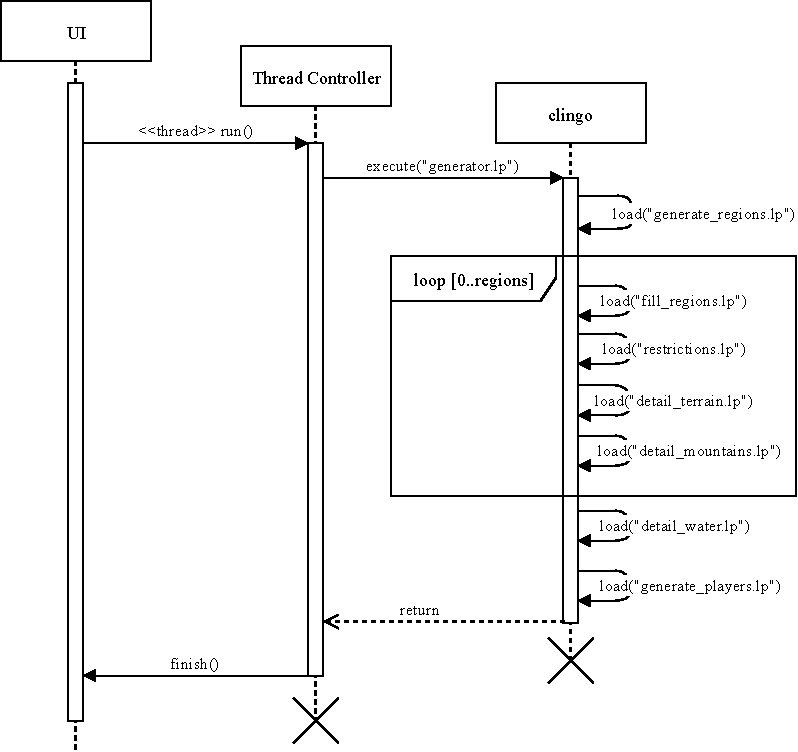
\includegraphics[width=\textwidth]{images/secuencia.pdf}
	\caption{Diagrama de secuencia de la ejecución del generador}
	\label{fig:sequence}
\end{figure}

\subsection{Implementación}
\label{subsec:implementacion}

Una vez analizado el proyecto en cuestión, pasaré a detallar el diseño de cada uno de los diferentes componentes del sistema en su construcción, indicando mediante diagramas como se integran los diferentes elementos. \\

Como ya se indicó en la Sección \ref{subsec:lua}, el lenguaje de programación Lua no tiene un paradigma de programación orientado a objetos basados en clases, más se ha preferido que en la realización de este sistema se use el módulo \textit{class.lua} de la biblioteca \textit{HUMP}\footnote{https://github.com/vrld/hump} para una organización lo más estructurada posible. Así mismo, también hay que destacar que el lenguaje tampoco soporta la manipulación de archivos en formato JSON, por lo que se ha usado el módulo \textit{json.lua}\footnote{https://github.com/rxi/json.lua}, el cual permite transformar un texto en formato JSON a tipos compatibles en Lua. \\

Por último, indicar que para la realización de las vistas de la interfaz de usuario se ha usado la biblioteca \textit{SUIT}\footnote{https://github.com/vrld/SUIT}, que permite generar una interfaz gráfica en modo inmediato de forma sencilla sobre LÖVE, pudiendo realizar un prototipo de los elementos más rápidamente y con más flexibilidad que con otro tipo de bibliotecas gráficas, como puede ser GTK+\footnote{https://www.gtk.org/}. Por otra parte, habrá elementos gráficos más complejos (como pueden ser diálogos de selección de ficheros o ventanas emergentes) que se tendrán que generar a mano, tal y como se expone en la Sección \ref{subsubsec:widgets}.

\subsubsection{Clase principal}
\label{subsubsec:main}

\begin{figure}[!h]
	\centering
	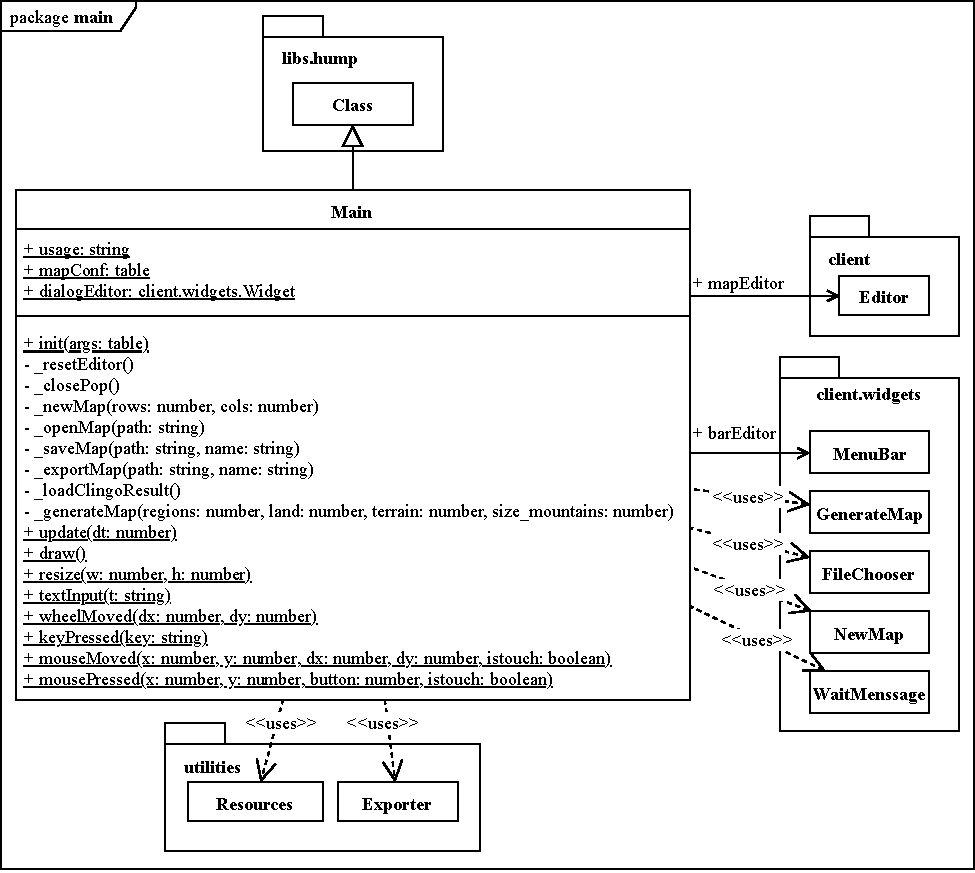
\includegraphics[width=\textwidth]{images/clase-principal.pdf}
	\caption{Diagrama de clases del paquete principal}
	\label{fig:mainclass}
\end{figure}

Como se puede ver en la Figura \ref{fig:mainclass} se ha diseñado la clase principal \texttt{Main}, la cual es una clase estática que sirve de controlador para las vistas y el modelo. Implementa los casos de uso de la interfaz descritos en la Sección \ref{subsec:cases} en los métodos \texttt{\_newMap}, \texttt{\_openMap}, \texttt{\_saveMap}, \texttt{\_exportMap} y \texttt{\_generateMap}, que son eventos que se llaman desde los diálogos emergentes tal y como se explica desde la Sección \ref{subsubsec:widgets}. Para el caso de uso de modificar el mapa, la tarea recae en la clase \texttt{Editor}, que se explica en detalle en la Sección \ref{subsubsec:client}. \\

Con respecto al motor gráfico LÖVE, este usa varias funciones predefinidas cuando se activan distintos eventos, los cuales llaman a los métodos públicos de la clase principal:

\begin{itemize}
	\item El método \texttt{init} es llamado en la función \texttt{love.load} la primera vez que se ejecuta el programa. Sirve para cargar los elementos gráficos e iniciar el resto de clases que serán usadas por el programa.
	\item Como LÖVE es un motor para programación de videojuegos, la función \texttt{love.update} es llamada en un bucle de eventos internos antes de actualizar la pantalla. Esta función llama al método homónimo de la clase principal, el cual prepara las vistas de la interfaz para su pintado en pantalla y llama a los métodos correspondientes según los eventos producidos en las vistas.
	\item Una vez actualizada la lógica, se procede al pintado de pantalla mediante la función \texttt{love.draw}, la cual llama al método con el mismo nombre de la clase principal, que se encarga de pintar las vistas en pantalla.
	\item Existen otros eventos, los cuales LÖVE tiene contempladas varias funciones por defecto adicionales que se lanzan para contestar a estos. Es el caso de cuando se redimensiona la ventana (\texttt{love.resize}), se introduce un texto mediante un teclado virtual (\texttt{love.textinput}), se realiza un movimiento de la rueda del ratón (\texttt{love.wheelmoved}), se presiona una tecla (\texttt{love.keypressed}), se mueve el ratón (\texttt{love.mousemoved}) o se presiona un botón del ratón (\texttt{love.mousepressed}). Estas llaman a los métodos correspondientes de la clase principal.
\end{itemize}

\subsubsection{Editor gráfico}
\label{subsubsec:client}

\begin{figure}[!h]
	\centering
	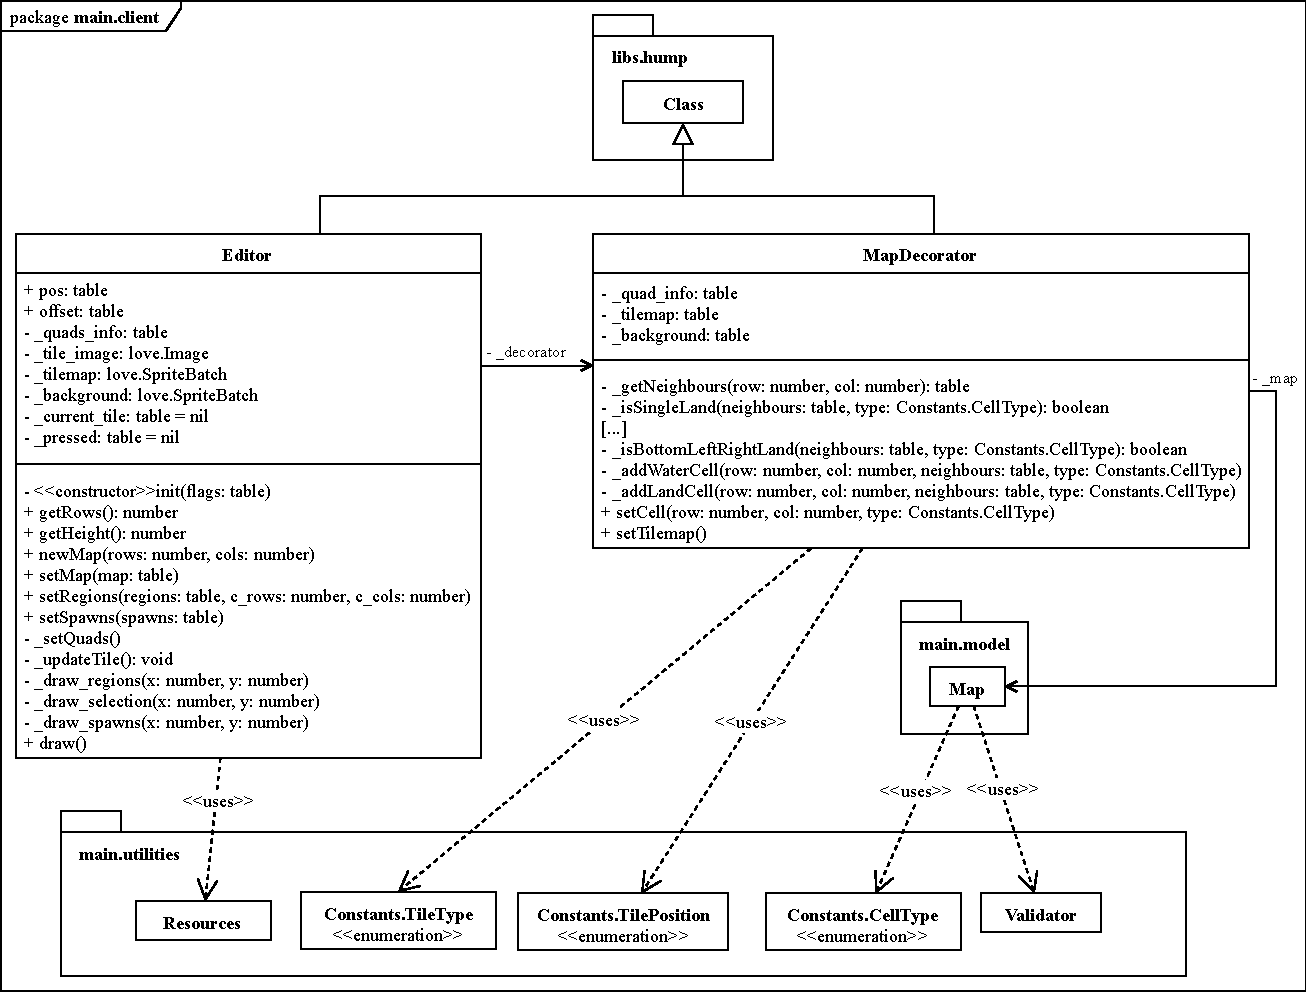
\includegraphics[width=\textwidth]{images/clase-editor.pdf}
	\caption{Diagrama de clases del paquete \texttt{Client}}
	\label{fig:editorclass}
\end{figure}

La clase \texttt{Editor} sirve como un controlador para responder a las modificaciones y cambios de representación del mapa, ya sea cuando se actualiza este mediante uno de los casos de uso que recoge la clase principal [ver Sección \ref{subsubsec:main}] o cuando el usuario procede a la modificación del mapa, tal y como se explica en la Sección \ref{subsec:cases}. \\

Para ello, siguiendo el patrón decorador, esta se apoya en la clase \texttt{MapDecorator}, la cual se encarga de actualizar la vista del mapa, que es representada mediante una rejilla con los distintos terrenos mediante el objeto \texttt{love.SpriteBatch}, el cual es un mapa de \textit{tiles} bidimensional. Debido a que hay terrenos que contienen diferentes imágenes para las posiciones de un \textit{tile}, \texttt{MapDecorator} contiene varios métodos que permiten discretizarlas conociendo los vecinos de una celda. Finalmente esta clase llama al modelo en si, representado por la clase \texttt{Map}, la cual tiene una representación del mapa en forma de tabla. \\

Finalmente todas estas clases usan constantes que están definidas el módulo \texttt{Constants}.

\subsubsection{Elemento gráficos complejos}
\label{subsubsec:widgets}

\begin{figure}[!h]
	\centering
	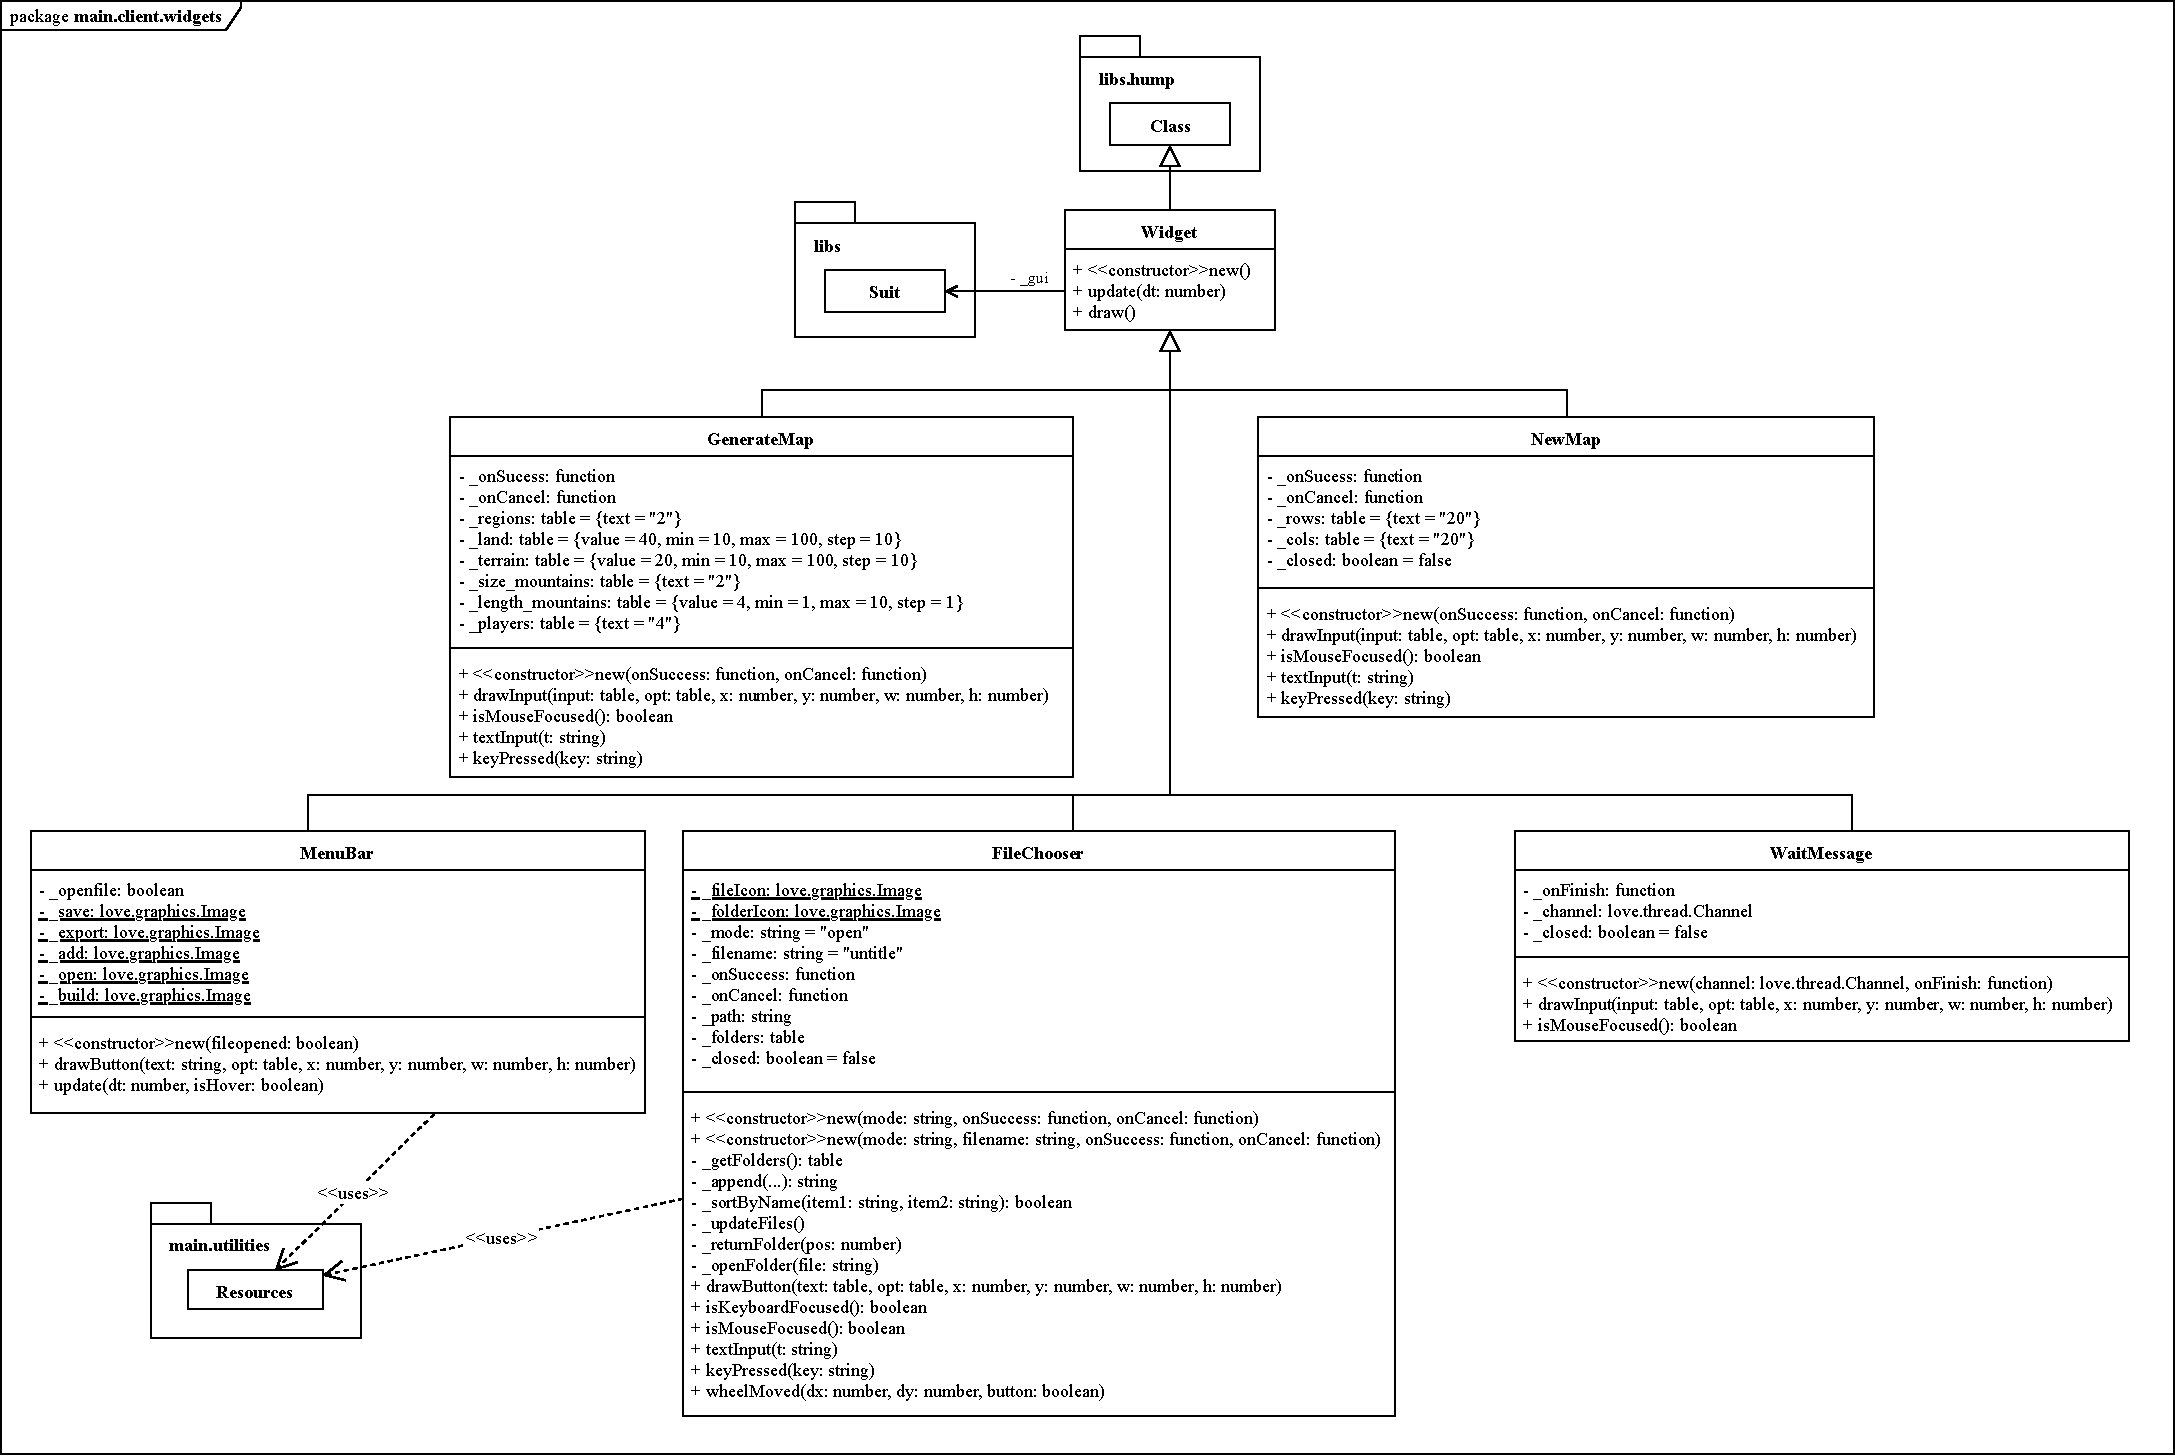
\includegraphics[width=\textwidth]{images/clases-widgets.pdf}
	\caption{Diagrama de clases del paquete \texttt{Widget}}
	\label{fig:widgetclasses}
\end{figure}

Como ya expliqué en la entrada de la Sección \ref{subsec:implementacion}, debido a las limitaciones de la biblioteca \textit{SUIT}, hay varios elementos gráficos que no se incluyen en ella debido a que son complejos y no es del ámbito de esta bibloteca, es por eso que se han realizado a mano. Estos elementos tienen su propio controlador para poder usarlos más fácilmente dentro del programa.

\begin{itemize}
	\item Para la barra de herramientas se ha realizado la clase \texttt{MenuBar}, la cual controla y muestra la lista de botones que accionan los principales casos de uso. Al constructor se le pasa las funciones para los eventos de aceptar y cancelar diálogo. Tiene un método \texttt{update} que devuelve un número que se corresponde con el botón pulsado en la barra.
	\item La clase \texttt{NewMap} controla y muestra la ventana emergente que se puede ver en la Figura \ref{fig:newmock}. Al constructor se le pasa las funciones para los eventos de aceptar y cancelar diálogo. Contiene el método \texttt{isMouseFocused} que indica si el ratón está encima de la ventana, y los métodos \texttt{textInput} y \texttt{keyPressed} para introducir texto en las entradas de la ventana.
	\item La clase \texttt{GenerateMap} controla y muestra la ventana emergente con el diálogo de generar mapa, tal y como se puede ver en la Figura \ref{fig:generatemock}. Contiene los mismos métodos que la clase \texttt{NewMap}.
	\item La clase \texttt{WaitMessage} controla y muestra la ventana emergente que se puede ver en la Figura \ref{fig:waitingmock}. Al constructor se le pasa el canal del \textit{thread} que se usa en la generación del mapa, tal y como se expone en la Sección \ref{subsubsec:generator}, y la función que se lanza cuando la generación termina. Contiene el método \texttt{isMouseFocused} que indica si el ratón está encima de la ventana.
	\item La clase \texttt{FileChooser} controla y muestra la ventana emergente correspondiente a un diálogo de selección de archivo, tal y como se puede ver en las Figuras \ref{fig:openmock}, \ref{fig:savemock} y \ref{fig:exportmock}. Contiene varios métodos privados para la ordenación y la apertura de carpetas en disco, así como el método \texttt{isMouseFocused} que indica si el ratón está encima de la ventana, los métodos \texttt{textInput} y \texttt{keyPressed} para introducir texto en las entradas de la ventana y el método \texttt{wheelMoved} que permite subir y bajar la lista de carpetas y ficheros mediante la rueda del ratón.
\end{itemize}